\documentclass{aip-cp}


\usepackage[numbers]{natbib}
\usepackage{rotating}
\usepackage{graphicx}

%% ДЛЯ РУССКОГО ТЕКСТА закомментировать потом!
\usepackage{inputenc}
\usepackage[T2A,T1]{fontenc}
\usepackage[english,russian]{babel}
\usepackage{cmap}
%%


% Document starts
\begin{document}

% Title portion
\title{Title}

\author[aff1]{Konstantin Barkalov\corref{cor1}}
\author[aff1]{Marina Usova}

\affil[aff1]{Lobachevsky State University of Nizhny Novgorod, Nizhny Novgorod, Russia}
\corresp[cor1]{Corresponding author: konstantin.barkalov@itmm.unn.ru}

\maketitle

\begin{abstract}
The paper presents results ...
\end{abstract}

% Head 1
\section{INTRODUCTION}

В настоящее время методы глобальной оптимизации используются для решения широкого круга задач, возникающих в различных областях науки и техники. 

Например, традиционной сферой применения методов глобальной оптимизации является идентификация значений параметров математических моделей по данным экспериментов. К их числу относятся, например, inverse problems of chemical kinetics.  В задачах такого вида требуется провести поиск значений неизвестных параметров модели, при которых результаты моделирования наиболее близки к результатам, полученным экспериментально.

Число параметров, которые требуется идентифицировать подобным образом, для задач химической кинетики может составлять десятки и сотни. Использование детерминированных методов глобальной оптимизации для решения задачах такой размерности крайне ограничено из-за чрезвычайно больших вычислительных затрат на покрытие search domain точками испытаний. Это остается справедливым даже в случае использования эффективных алгоритмов (например, \cite{Paulavicius2011,Evtushenko2009,Jones2009}), строящих существенно неравномерные покрытия. 

Многие обратные задачи характеризуются тем, что зависимость от разных групп параметров носит разный характер. Например, от одной группы параметров зависимость может быть близка к линейной, тогда как по второй группе зависимость может носить сложный многоэкстремальный характер.

В этом случае решение задачи можно организовать по схеме recursive optimization. Решение  многоэкстремальной подзадачи, для которой требуется использовать сложные алгоритмы глобальной оптимизации, будет проводиться на верхнем уровне рекурсии.
Унимодальные подзадачи (каждая из которых соответствует фиксированному набору значений первой части параметров) будут решаться на нижнем уровне. Для их решения можно применять обладающие быстрой сходимостью методы локальной оптимизации.

Однако заранее указать разделение на группы параметров с разным характером поведения целевой функции, как правило, не представляется возможным, т.к. целевая функция в обратных задачах задается как черный ящик. 
Таким образом, актуальной является разработка алгоритмов минимизации существенно многомерных функций, в которых учитывается разный характер зависимости целевой функции от разных групп параметров. 
В данной работе предложен конкретный механизм такого разделения, основанный на <указать>.
В качестве примеров, подтверждающих работоспособность предложенной схемы, решены как тестовые, так и прикладные задачи.

\section{GLOBAL SEARCH ALGORITHM}


The global optimization problem \cite{Strongin2000}


\section{NUMERICAL EXPERIMENTS}

The calculations were performed on the computer cluster of the Institute for Systems Programming and the UniHub web-lab \cite{UniHub}. The web-lab architecture is based on the cloud computing model where resources (servers, networks, storage systems, applications, etc.) are provided remotely as a set of different-level services with on-demand servicing.

%\begin{figure}%[ht]
%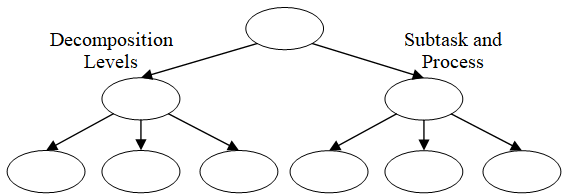
\includegraphics[width=1.0\linewidth]{fig1.png}
%\caption{Schematic representation of the computational domain, with the geometry parameterization points marked in red and the black points independent of the optimization iterations. The grey lines show the possible deformation of the geometry.}
%\label{fig}
%\end{figure}

The calculation was carried out ...

% Acknowledgement
\section{ACKNOWLEDGMENTS}
This study was supported by the Russian Science Foundation, project No 21-11-00204.



% References

%\nocite{*}
\bibliographystyle{aipnum-cp}%
\bibliography{bibliography}%


\end{document}
